% Options for packages loaded elsewhere
\PassOptionsToPackage{unicode}{hyperref}
\PassOptionsToPackage{hyphens}{url}
\PassOptionsToPackage{dvipsnames,svgnames,x11names}{xcolor}
%
\documentclass[
  a4paper,
]{scrreport}

\usepackage{amsmath,amssymb}
\usepackage{iftex}
\ifPDFTeX
  \usepackage[T1]{fontenc}
  \usepackage[utf8]{inputenc}
  \usepackage{textcomp} % provide euro and other symbols
\else % if luatex or xetex
  \usepackage{unicode-math}
  \defaultfontfeatures{Scale=MatchLowercase}
  \defaultfontfeatures[\rmfamily]{Ligatures=TeX,Scale=1}
\fi
\usepackage{lmodern}
\ifPDFTeX\else  
    % xetex/luatex font selection
\fi
% Use upquote if available, for straight quotes in verbatim environments
\IfFileExists{upquote.sty}{\usepackage{upquote}}{}
\IfFileExists{microtype.sty}{% use microtype if available
  \usepackage[]{microtype}
  \UseMicrotypeSet[protrusion]{basicmath} % disable protrusion for tt fonts
}{}
\makeatletter
\@ifundefined{KOMAClassName}{% if non-KOMA class
  \IfFileExists{parskip.sty}{%
    \usepackage{parskip}
  }{% else
    \setlength{\parindent}{0pt}
    \setlength{\parskip}{6pt plus 2pt minus 1pt}}
}{% if KOMA class
  \KOMAoptions{parskip=half}}
\makeatother
\usepackage{xcolor}
\setlength{\emergencystretch}{3em} % prevent overfull lines
\setcounter{secnumdepth}{-\maxdimen} % remove section numbering
% Make \paragraph and \subparagraph free-standing
\ifx\paragraph\undefined\else
  \let\oldparagraph\paragraph
  \renewcommand{\paragraph}[1]{\oldparagraph{#1}\mbox{}}
\fi
\ifx\subparagraph\undefined\else
  \let\oldsubparagraph\subparagraph
  \renewcommand{\subparagraph}[1]{\oldsubparagraph{#1}\mbox{}}
\fi


\providecommand{\tightlist}{%
  \setlength{\itemsep}{0pt}\setlength{\parskip}{0pt}}\usepackage{longtable,booktabs,array}
\usepackage{calc} % for calculating minipage widths
% Correct order of tables after \paragraph or \subparagraph
\usepackage{etoolbox}
\makeatletter
\patchcmd\longtable{\par}{\if@noskipsec\mbox{}\fi\par}{}{}
\makeatother
% Allow footnotes in longtable head/foot
\IfFileExists{footnotehyper.sty}{\usepackage{footnotehyper}}{\usepackage{footnote}}
\makesavenoteenv{longtable}
\usepackage{graphicx}
\makeatletter
\def\maxwidth{\ifdim\Gin@nat@width>\linewidth\linewidth\else\Gin@nat@width\fi}
\def\maxheight{\ifdim\Gin@nat@height>\textheight\textheight\else\Gin@nat@height\fi}
\makeatother
% Scale images if necessary, so that they will not overflow the page
% margins by default, and it is still possible to overwrite the defaults
% using explicit options in \includegraphics[width, height, ...]{}
\setkeys{Gin}{width=\maxwidth,height=\maxheight,keepaspectratio}
% Set default figure placement to htbp
\makeatletter
\def\fps@figure{htbp}
\makeatother

%\newfontfamily\Ubuntu[Mapping=tex-text]{Ubuntu}
\usepackage{pgfplots}
\usetikzlibrary{arrows.meta,arrows}
\usetikzlibrary{angles,quotes}
\pgfplotsset{grid style={dashed,mygray}}
% Colors
\definecolor{myblue}{rgb}{0.067,0.529,0.871}
\definecolor{mypurple}{rgb}{0.859,0.071,0.525}
\definecolor{myred}{rgb}{1.0, 0.13, 0.32}
\definecolor{mygreen}{rgb}{0.01, 0.75, 0.24}
\definecolor{myblack}{gray}{0.1}
\definecolor{mygray}{gray}{0.8}
\newcommand{\NN}{\mathbb{N}}
\newcommand{\ZZ}{\mathbb{Z}}
\newcommand{\QQ}{\mathbb{Q}}
\newcommand{\RR}{\mathbb{R}}
\newcommand{\CC}{\mathbb{C}}
\DeclareMathOperator{\Int}{Int}
\DeclareMathOperator{\Ext}{Ext}
\DeclareMathOperator{\Fr}{Fr}
\DeclareMathOperator{\Adh}{Adh}
\DeclareMathOperator{\Ac}{Ac}
\DeclareMathOperator{\sen}{sen}
\makeatletter
\makeatother
\makeatletter
\makeatother
\makeatletter
\@ifpackageloaded{caption}{}{\usepackage{caption}}
\AtBeginDocument{%
\ifdefined\contentsname
  \renewcommand*\contentsname{Indice de contenidos}
\else
  \newcommand\contentsname{Indice de contenidos}
\fi
\ifdefined\listfigurename
  \renewcommand*\listfigurename{Listado de Figuras}
\else
  \newcommand\listfigurename{Listado de Figuras}
\fi
\ifdefined\listtablename
  \renewcommand*\listtablename{Listado de Tablas}
\else
  \newcommand\listtablename{Listado de Tablas}
\fi
\ifdefined\figurename
  \renewcommand*\figurename{Figura}
\else
  \newcommand\figurename{Figura}
\fi
\ifdefined\tablename
  \renewcommand*\tablename{Tabla}
\else
  \newcommand\tablename{Tabla}
\fi
}
\@ifpackageloaded{float}{}{\usepackage{float}}
\floatstyle{ruled}
\@ifundefined{c@chapter}{\newfloat{codelisting}{h}{lop}}{\newfloat{codelisting}{h}{lop}[chapter]}
\floatname{codelisting}{Listado}
\newcommand*\listoflistings{\listof{codelisting}{Listado de Listados}}
\makeatother
\makeatletter
\@ifpackageloaded{caption}{}{\usepackage{caption}}
\@ifpackageloaded{subcaption}{}{\usepackage{subcaption}}
\makeatother
\makeatletter
\@ifpackageloaded{tcolorbox}{}{\usepackage[skins,breakable]{tcolorbox}}
\makeatother
\makeatletter
\@ifundefined{shadecolor}{\definecolor{shadecolor}{rgb}{.97, .97, .97}}
\makeatother
\makeatletter
\makeatother
\makeatletter
\makeatother
\ifLuaTeX
\usepackage[bidi=basic]{babel}
\else
\usepackage[bidi=default]{babel}
\fi
\babelprovide[main,import]{spanish}
% get rid of language-specific shorthands (see #6817):
\let\LanguageShortHands\languageshorthands
\def\languageshorthands#1{}
\ifLuaTeX
  \usepackage{selnolig}  % disable illegal ligatures
\fi
\IfFileExists{bookmark.sty}{\usepackage{bookmark}}{\usepackage{hyperref}}
\IfFileExists{xurl.sty}{\usepackage{xurl}}{} % add URL line breaks if available
\urlstyle{same} % disable monospaced font for URLs
\hypersetup{
  pdftitle={Envío de mensajes en una red de telefonía móvil},
  pdflang={es},
  colorlinks=true,
  linkcolor={blue},
  filecolor={Maroon},
  citecolor={Blue},
  urlcolor={Blue},
  pdfcreator={LaTeX via pandoc}}

\title{Envío de mensajes en una red de telefonía móvil}
\author{}
\date{}

\begin{document}
\begin{titlepage}

%\AddToShipoutPicture*{\put(0,0){\includegraphics[scale=0.8]{img/background2}}} % Imagen de fondo, requiere el paquete eso-pic.
\begin{center}
\vspace*{5cm}

\Huge
{\textbf{\textsf{Envío de mensajes en una red de telefonía móvil}}}

\vspace{0.5cm}
\LARGE
{\textbf{\textsf{}}}

\vspace{1.5cm}


\includegraphics[width=0.4\textwidth]{../img/logos/proyectos.png}
\end{center}

\vfill

\begin{flushleft}
\begin{tabular}{ll}

\includegraphics[width=0.1\textwidth]{../img/logos/aprendeconalf.png} & \parbox[b]{5cm}{\Large\textsf{}\\ \textsf{asalber@ceu.es} \\ \textsf{https://aprendeconalf.es}}
\end{tabular}
\end{flushleft}
\end{titlepage}\ifdefined\Shaded\renewenvironment{Shaded}{\begin{tcolorbox}[interior hidden, breakable, borderline west={3pt}{0pt}{shadecolor}, sharp corners, enhanced, frame hidden, boxrule=0pt]}{\end{tcolorbox}}\fi

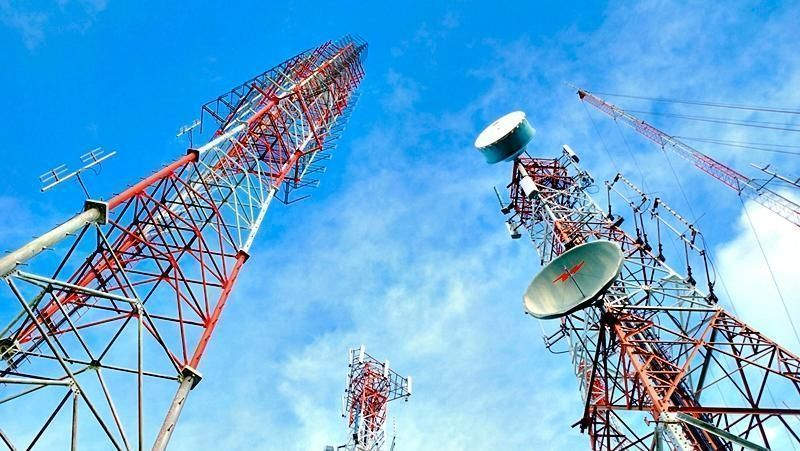
\includegraphics{../img/telefonia-movil/antenas.jpg}

\hypertarget{introducciuxf3n}{%
\section{Introducción}\label{introducciuxf3n}}

La telefonía móvil utiliza una red de estaciones y subestaciones de
telecomunicación 4G para la transmisión de datos entre dispositivos
móviles. Muchas de estas estaciones están interconectadas por fibra y
otras se comunican mediante conexiones inalámbricas por radio
frecuencias.

Para que un mensaje llegue de un dispositivo emisor a otro receptor, el
mensaje debe recorrer el camino que va de la subestación más próxima al
emisor a la más próxima al receptor, pasando, a menudo, por varias
estaciones de la red que interconectan las subestaciones de origen y
destino. La distancia entre las estaciones y su capacidad de transmisión
de datos son claves para que los mensajes lleguen lo más rápidamente
posible del dispositivo emisor al receptor.

\hypertarget{objetivos}{%
\section{Objetivos}\label{objetivos}}

En este proyecto se debe desarrollar un algoritmo y una aplicación para
buscar el camino óptimo para enviar un mensaje desde un punto geográfico
a otro de una ciudad a través del grafo que representa la red de
estaciones y subestaciones de telecomunicación de la ciudad.

La aplicación recibirá como entrada las coordenadas de los puntos de
origen y destino, y el tamaño del mensaje, y debe devolver el camino más
rápido para enviar el mensaje del origen al destino, es decir, el orden
de las estaciones por las que el mensaje debe pasar, así como el tiempo
que el mensaje tardaría en recorrer ese camino. En la búsqueda del
camino óptimo debe tenerse en cuenta la distancia entre las
subestaciones, así como la capacidad de transmisión de cada una de
ellas.

Para la búsqueda del camino óptimo en el grafo conviene utilizar el
famoso
\href{https://es.wikipedia.org/wiki/Algoritmo_de_Dijkstra}{algoritmo de
Dijkstra} o alguna de sus variantes.

\hypertarget{tareas}{%
\section{Tareas}\label{tareas}}

\begin{enumerate}
\def\labelenumi{\arabic{enumi}.}
\tightlist
\item
  Obtener las coordenadas geográficas de la ubicación de las estaciones
  de telefonía con una frecuencia específica y de un único operador en
  una determinada ciudad y representar la red en un plano cartesiano. Se
  puede asumir que las estaciones a menos de \(x\) kilómetros de
  separación están directamente conectadas por fibra.
\item
  Construir un grafo que represente la red de estaciones de telefonía.
  Los pesos de las aristas del grafo podrían ser las distancias en línea
  recta entre las estaciones, pero es mucho más realista es utilizar la
  velocidad de conexión entre ellas en Mbps, ya que las estaciones base
  suelen conectarse entre ellas con conexiones inalámbricas. Para ello
  se puede utilizar la capacidad de Shannon como se explica en este
  \href{https://dspace.networks.imdea.org/bitstream/handle/20.500.12761/689/main_Throughput_MiSARN2019_CameraReady_Embedded_CertifiedIEEEeXplore.pdf?sequence=1}{artículo}.
\item
  Identificar en el grafo las estaciones base más cercanas a las
  coordenadas de los puntos de origen y destino del mensaje.
\item
  Implementar en Python o Julia el algoritmo de Dijkstra o alguna de sus
  variantes para la búsqueda del camino óptimo.
\item
  Determinar cuál será la estación base que requiera más atención de
  mantenimiento, es decir, por la que pasen más mensajes. Para ello,
  usar la métrica de centralidad correspondiente. O lo que es lo mismo,
  si hubiera un agente malicioso (a.k.a. man in the middle, o Charlie),
  ¿dónde se ubicaría para interceptar la mayoría de mensajes.
\item
  Determinar cuánto tardará como máximo un mensaje en llegar de emisor a
  receptor. Usar la matriz de distancias tras ejecutar el algoritmo de
  Dijkstra y calcular el diámetro del grafo.
\end{enumerate}

\hypertarget{datos}{%
\section{Datos}\label{datos}}

Para probar obtener los datos de la ubicación y frecuencia de
transmisión de las estaciones de telefonía de una determinada ciudad
puede consultarse
\href{https://geoportal.minetur.gob.es/VCTEL/vcne.do}{web del Ministerio
de Asuntos Económicos y Transformación Digital} o bien esta otra web con
el \href{https://antenasgsm.com/}{mapa de estaciones de telefonía del
Estado español}.



\end{document}
